\chapter{Embedded Visualizations in ICE}
\label{sec:embeddedViz}

\section{Introduction}\label{introduction}

This document describes the embedded visualization capabilities
available in ICE. Embedded visualizations in ICE aim to provide users
with immediate yet simple visualization of simulation input and output
well within the simulation workflow. In other words, simulation input
and output can be visually verified or validated without leaving the
associated Model Builder or Job Launcher in ICE. For more advanced or
complex visualization tasks in ICE, please see the document on
\href{Visualizing Output with ICE}{Visualizing Output with ICE}.

\section{Resources and Resource
Pages}\label{resources-and-resource-pages}

ICE \emph{Items} may include any number of \emph{Resources}, which may
include any type of file like meshes, pictures, shell scripts,
\texttt{.csv} files, or even plain text files. For example, a
\emph{Model Builder}, which is used in ICE to configure simulation
input, may at some point include a plain text input file as well as
associated data files or meshes. Likewise, a \emph{Job Launcher}, which
actually launches the simulation, may produce any type of output data,
which may also include \texttt{.csv} files, binary files, or even more
mesh files.

Before proceeding, you should familiarize yourself with the
\emph{Resources View} (highlighted in blue on the left) and the idea of
a \emph{Resource Page} (highlighted in red, while its tab is highlighted
at the bottom) as shown in the image below.

\begin{figure}[htbp]
\centering
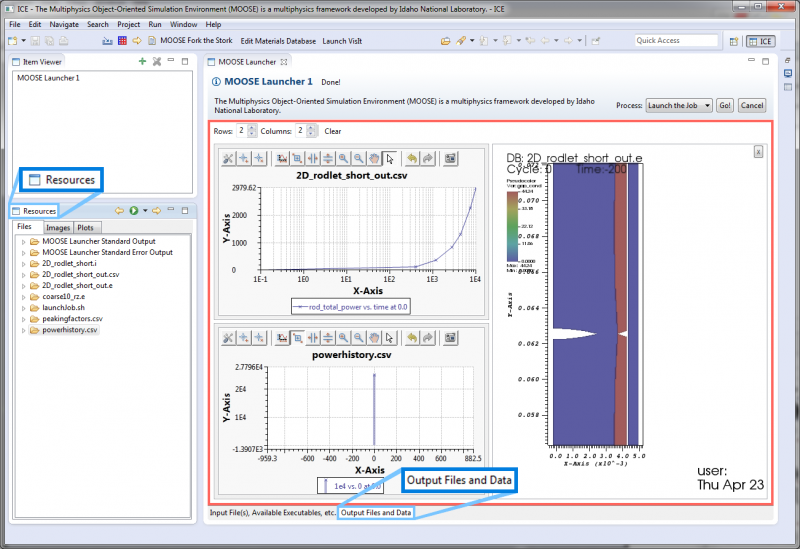
\includegraphics[width=\textwidth]{figures/ICE_Viz_ResourceViewPage.png}
\caption{The new ICE Resource View showing generated output files that can be visualized natively in the view. }
\end{figure}

\subsubsection{The Resources View}\label{the-resources-view}

Some \emph{Items} in ICE store references to these resources for easy
access to the user. In these cases, the resources are presented to the
user in the \emph{Resources View}, which is part of the default ICE
perspective.

The \emph{Resource View} is actually a tree, where each resource has its
own node. If you expand a resource node, it will reveal the underlying
file's path along with its date of last modification.

\subsubsection{Resource Pages}\label{resource-pages}

If an ICE \emph{Item} includes resources, it will have a designated tab
for showing those resources.

\begin{itemize}
\itemsep1pt\parskip0pt\parsep0pt
\item
  For \emph{Model Builders}, this tab could be named anything. For
  instance, in the \emph{MOOSE Model Builder}, the tab for viewing
  resources is called \emph{Mesh}.
\item
  For \emph{Job Launchers}, this tab will be named \emph{Output Files
  and Data}.
\end{itemize}

Click on the tab to open it and view the \emph{Item}'s \emph{Resource
Page}. Each \emph{Resource Page} is capable of showing plain text files
or embedded visualizations based on the selected resource's file type.

\subsubsection{Viewing a Resource}\label{viewing-a-resource}

To open a resource, go to the \emph{Resources View} and double-click its
item in the list of available resources. The way ICE handles this
selected resource depends on the following:

\begin{enumerate}
\itemsep1pt\parskip0pt\parsep0pt
\item
  If the file can be opened using one of the visualization services, it
  will be added to the active \emph{Resource Page}.
\item
  If the file can be opened using a plain text editor, it will be opened
  in a new \emph{Text Editor} in ICE.
\item
  If the file cannot be opened, the \emph{Resource Page} will attempt to
  render it through a browser widget. This handles some basic files like
  certain image types.
\item
  If the file cannot be opened in the browser, the browser will prompt
  you to save the file. In this case, you can either save it, or cancel
  and open the existing file at the location specified in the
  \emph{Resources View}.
\end{enumerate}

This document will not discuss the latter three situations any further.
The next sections will describe the embedded visualizations from the
first scenario.

\subsubsection{Controlling Embedded
Visualizations}\label{controlling-embedded-visualizations}

Each \emph{Resource Page} can display a number of embedded
visualizations at any time. Selected plots are displayed in a grid
defined by the \emph{Rows} and \emph{Columns} widgets in the toolbar
(highlighted in blue in the image below) near the top of the page,
although embedded plots will take up as much space as they can. The
default grid is two by two, although the number of rows and columns can
be changed at any time.

\begin{figure}[htbp]
\centering
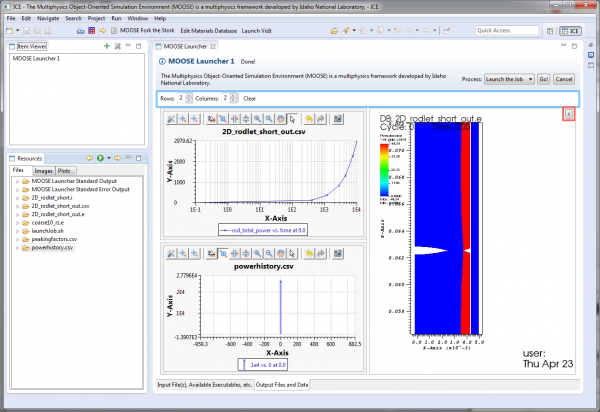
\includegraphics[width=\textwidth]{figures/ICE_Viz_Grid.png}
\caption{The Resource Page grid of plots can be modified through the rows/columns toggle buttons.}
\end{figure}

\paragraph{Adding Plots to the Grid}\label{adding-plots-to-the-grid}

To add a new plot to the grid, simply go to the \emph{Resources View}
and double-click the desired file that can be rendered by one of ICE's
visualization services. Note that the order in which plots appear in the
grid depend on the order in which they are added to the grid, with the
grid moving left-to-right, top-to-bottom.

\paragraph{Removing Plots from the
Grid}\label{removing-plots-from-the-grid}

To remove an individual plot, you have two choices:

\begin{enumerate}
\itemsep1pt\parskip0pt\parsep0pt
\item
  You can hover the mouse cursor over the plot, then click the ``X''
  button that appears (highlighted in red in the image above).
\item
  You can right-click somewhere inside the plot, then click
  \emph{Remove}.
\end{enumerate}

You can also remove all plots at once by clicking the \emph{Clear}
button in the \emph{Resource Page}'s toolbar. This is located next to
the widgets for controlling the size of the grid.

\paragraph{Right-click Menus}\label{right-click-menus}

Every plot drawn inside the \emph{Resource Page} includes a right-click
menu that provides the following basic options:

\begin{enumerate}
\itemsep1pt\parskip0pt\parsep0pt
\item
  \textbf{Remove} - Removes the plot from the \emph{Resource Page}
\item
  \textbf{Set Plot Type} - Provides nested sub-menus that let you set
  what is displayed in the plot.
\end{enumerate}

The contents of the \emph{Set Plot Type} sub-menu depends on both the
file and the visualization service used to plot it. Generally, you first
choose the plot \emph{category} from the first sub-menu and then a
\emph{type} from the category sub-menu.

Additional menu choices may be available depending on the visualization
service that provides the plot.

\section{Visualization Services}\label{visualization-services}

\subsubsection{VisIt}\label{visit}

\paragraph{Prerequisites}\label{prerequisites}

To use the embedded visualization service for \emph{VisIt}, ICE requires
a local installation of
\href{https://wci.llnl.gov/simulation/computer-codes/visit/}{VisIt}
(minimum version 2.8.2) developed by Lawrence Livermore National
Laboratory.

\paragraph{Preferences}\label{preferences}

\subparagraph{Getting to the
Preferences}\label{getting-to-the-preferences}

Using the \emph{VisIt} visualization service for viewing complex 2D or
3D mesh data requires little initial configuration. Assuming the
\hyperref[Prerequisites]{VisIt prerequisite} is installed, use the the
main menu bar at the top of the window and navigate to:

\emph{Window} \textgreater{} \emph{Preferences}

In the \emph{Preferences} dialog, navigate to:

\emph{Visualization} \textgreater{} \emph{VisIt} (highlighted in blue in
the image below)

\begin{figure}[htbp]
\centering
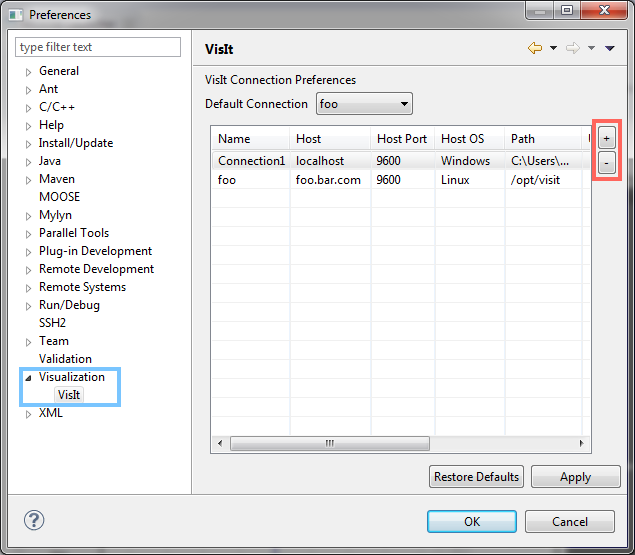
\includegraphics[width=\textwidth]{figures/ICE_Viz_VisIt_Preferences.png}
\caption{The new VisIt Preferences Page.}
\end{figure}

\subparagraph{Adding Connections}\label{adding-connections}

You will need to press the + button (highlighted above in red) to the
right of the table to add a new entry. Fill out the new row in the
table. Generally speaking, the default values are fine, but the
\emph{Path} will need to be updated to point to the folder containing
your VisIt executable. You can copy and paste the path into this field
and press \emph{Enter}.

\subparagraph{Setting the Default
Connection}\label{setting-the-default-connection}

Currently, only one connection to VisIt can be used at a time. If you
only have one configured connection, it is automatically selected as the
default. However, if you have multiple configured connections, you will
need to set the \emph{default} connection by choosing from the drop down
above the table.

\subparagraph{Removing Connections}\label{removing-connections}

To remove a connection, click on any cell in its row in the table, then
click the "-" button (highlighted above in red) on the right of the
table. You can select multiple connections by holding \emph{CTRL} while
you click them, then clicking the "-" button.

\subparagraph{Applying the Connection
Preferences}\label{applying-the-connection-preferences}

When you have finished updating your connection configurations for
VisIt, you can click \emph{OK} to apply the changes and close the
\emph{Preferences} dialog. Alternatively, you can apply the changes
immediately by clicking \emph{Apply}. It is then safe to close the
\emph{Preferences} dialog in any valid way, e.g., by clicking the
dialog's close button or by clicking \emph{Cancel}.

\paragraph{Opening a VisIt Plot}\label{opening-a-visit-plot}

The \emph{Resources View} will pass any ICE resources pointing to
\texttt{.e} (Exodus) or \texttt{.silo} files to the \emph{VisIt
Visualization Service}. If the visualization service is configured and
running and if the file is valid, then the \emph{Resource Page} will
open a view of the resource powered by the default VisIt connection, as
in the image of a battery mesh SILO file below.

An example VisIt plot embedded in a \emph{Model Builder} can be seen in Figure 2.4.

\begin{figure}[htbp]
\centering
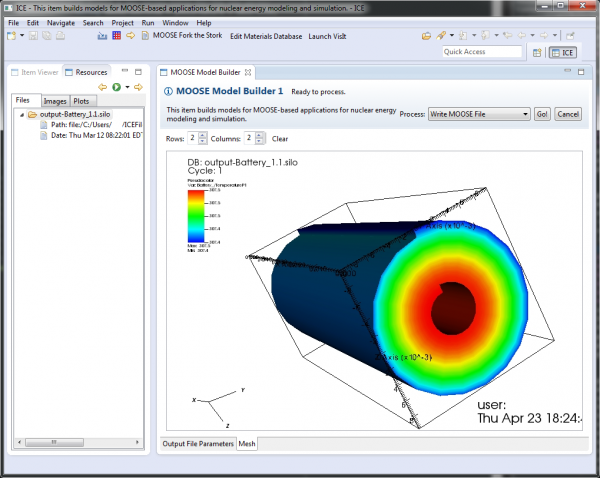
\includegraphics[width=\textwidth]{figures/ICE_Viz_VisIt.png}
\caption{An embedded VisIt plot in the MOOSE Model Builder. }
\end{figure}

The embedded VisIt view can be rotated by clicking and dragging and
zoomed in and out with the mouse wheel.

\paragraph{Right-click Menu}\label{right-click-menu}

The image below shows the context menu available when right-clicking
somewhere inside the VisIt view.

\begin{figure}[htbp]
\centering
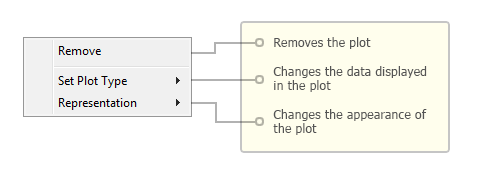
\includegraphics[scale=.6]{figures/ICE_Viz_VisIt-ContextMenu.png}
\caption{The embedded plot contains context-menu right-click functionality for modifying or deleting the plot.}
\end{figure}

The plot types available in the context menu depend on the data
available in the VisIt-compatible file. In the case of this SILO file,
the only plot categories are \emph{Meshes} and \emph{Scalars}.

The context menu also includes the ability to change how the VisIt plot
is rendered. The representations available depend on the current plot
type. A full list of supported ``representations'' is listed below for
each plot category.

\begin{itemize}
\itemsep1pt\parskip0pt\parsep0pt
\item
  Materials

  \begin{itemize}
  \itemsep1pt\parskip0pt\parsep0pt
  \item
    Boundary \emph{(default)}
  \item
    FilledBoundary
  \end{itemize}
\item
  Meshes

  \begin{itemize}
  \itemsep1pt\parskip0pt\parsep0pt
  \item
    Mesh \emph{(default)}
  \end{itemize}
\item
  Scalars

  \begin{itemize}
  \itemsep1pt\parskip0pt\parsep0pt
  \item
    Pseudocolor \emph{(default)}
  \item
    Contour
  \item
    Volume
  \end{itemize}
\item
  Vectors

  \begin{itemize}
  \itemsep1pt\parskip0pt\parsep0pt
  \item
    Vector \emph{(default)}
  \end{itemize}
\end{itemize}

\subsubsection{CSV}\label{csv}

\paragraph{Prerequisites}\label{prerequisites-1}

The embedded visualizations for \texttt{.csv} data require no additonal
software to be installed or any preference configuration.

\paragraph{Opening a CSV Plot}\label{opening-a-csv-plot}

The \emph{Resources View} will pass any ICE resources pointing to
\texttt{.csv} files to the \emph{CSV Visualization Service}. If the file
can be read by the \emph{CSV Visualization Service}, then the
\emph{Resource Page} will open a plot that contains the first available
series in the file.
An example CSV plot embedded in a \emph{Job Launcher} can be seen in Figure 2.6.

\begin{figure}[htbp]
\centering
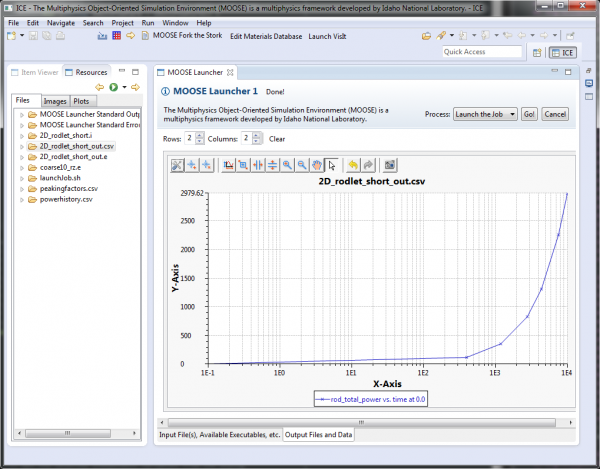
\includegraphics[width=\textwidth]{figures/ICE_Viz_CSV.png}
\caption{An embedded CSV plot in the MOOSE Launcher Resource Page, representing some MOOSE PostProcessor data.}
\end{figure}

The embedded CSV plot includes the same toolbar described in the the
standard features provided by the
\href{Visualizing_Output_with_ICE\#Plot_Toolbar}{\emph{CSV Plot Editor}
in the \emph{Visualization Perspective}} as well as a right-click menu
to modify the plot.

\paragraph{Right-click Menu}\label{right-click-menu-1}

The image below shows the context menu available when right-clicking
somewhere inside the CSV plot.

\begin{figure}[htbp]
\centering
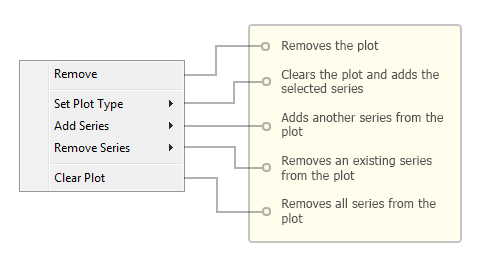
\includegraphics[width=\textwidth]{figures/ICE_Viz_CSV-ContextMenu.png}
\caption{The CSV context-menu. }
\end{figure}

By choosing a series from the \emph{Set Plot Type} sub-menu, you can
change what series is plotted. This will clear any existing series from
the plot and add the selected series.

To add more series to the plot, choose a series from the \emph{Add
Series} sub-menu.

To remove a plotted series, choose one of the existing series from the
\emph{Remove Series} sub-menu. This sub-menu will be disabled if there
are no series to remove.

To clear all series from the plot, click \emph{Clear Plot} at the bottom
of the menu.
